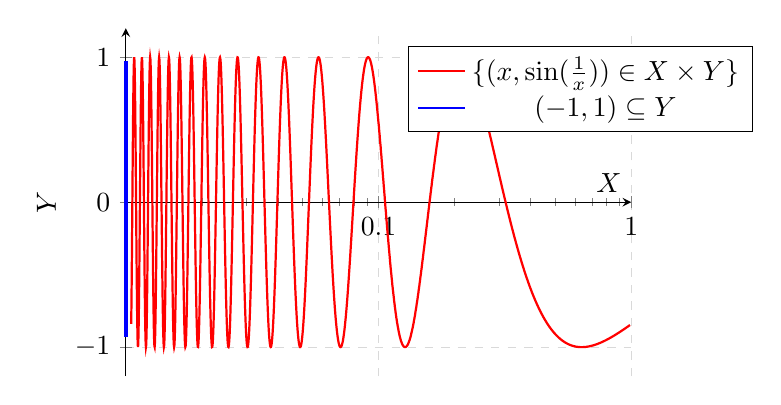
\begin{tikzpicture}
    \begin{axis}[
        axis x line=middle,
        axis y line=left,
        enlarge y limits=true,
        xmode=log, % Logarithmic x axis
        xmin=0.01, xmax=1, % Positive domain...
        xticklabel=\pgfmathparse{exp(\tick)}\pgfmathprintnumber{\pgfmathresult},
        xticklabel style={/pgf/number format/.cd,fixed}, % Use fixed point notation
        width=8cm, height=6cm,     % size of the image
        grid = major,
        grid style={dashed, gray!30},
        ymin=-1,      % start the diagram at this y-coordinate
        ymax= 1,      % end   the diagram at this y-coordinate
        axis background/.style={fill=white},
        ylabel=$Y$,
        xlabel=$X$,
        legend style={at={(0.9,0.95)}, anchor=north}
     ]
      \addplot[domain=0.0105:1, red, thick,samples=2000] {-sin(deg(1/(x)))};
      \addplot[domain=0.0105:0.011, blue, thick,samples=20] {10};
      \addlegendentry{$\{(x, \sin(\frac{1}{x})) \in X \times Y\}$}
      \addlegendentry{$(-1,1) \subseteq Y$}
    \end{axis}
      \draw[ultra thick,blue] (0,0.5) -- (0,4);
\end{tikzpicture}
